\documentclass[12pt,a4paper]{article}
\usepackage[utf8]{inputenc}
\usepackage[T1]{fontenc}
\usepackage{times}
\usepackage[margin=2.5cm]{geometry}
\usepackage{setspace}
\doublespacing
\usepackage{graphicx}
\usepackage{booktabs}
% natbib removed for Chicago notes-bibliography
\usepackage{hyperref}
\usepackage{amsmath}

\title{Temple Siting as Archaeological Proxy: Using Candi Distribution Patterns to Predict Buried Sites in Volcanic Java}

\author{Mukhlis Amien\textsuperscript{1} \and Go Frendi Gunawan\textsuperscript{1}}

\date{}

\begin{document}

\maketitle

\noindent\textsuperscript{1}Lab Data Sains, Universitas Bhinneka Nusantara, Malang, Indonesia

\vspace{1em}
\noindent\textbf{Corresponding author:} Mukhlis Amien (\texttt{amien@ubhinus.ac.id})

\begin{abstract}
Volcanic sedimentation in Java buries archaeological sites at rates of 3--13~mm/yr, creating systematic gaps in the pre-modern record. We propose using surviving Hindu-Buddhist temple (\emph{candi}) distributions as spatial proxies for undiscovered sites. Analysis of 142 candi reveals three exploitable patterns: (1) candi cluster on western volcanic flanks (Rayleigh $p=3.4\times10^{-8}$); (2) Zone A ($<$10~km from volcanic peaks) is overrepresented by 17.9$\times$; and (3) temple orientations follow canonical prescription ($85\%$ equinox-facing, $p=4.9\times10^{-14}$) while siting follows volcanic logic. Comparison with 170 georeferenced inscriptions confirms that this volcanic proximity is specific to sacred architecture: inscriptions are 9.2~km farther from volcanoes (Mann-Whitney $p=5.2\times10^{-8}$), demonstrating that temple siting reflects intentional landscape decisions, not general settlement geography. A dataset of 51 eruption-site correlations with measured burial depths (mean 3.41~m, max 9.14~m) independently confirms the severity of volcanic burial. An adversarial regression controlling for survey intensity confirms that the volcanic-zone site deficit is substantive ($p=0.0015$). Comparison with Japan---which has 100--200$\times$ greater survey intensity and finds buried volcanic sites through rescue archaeology---clarifies that the archaeological gap reflects the interaction of volcanic burial with insufficient survey investment, not volcanism alone. We derive ten fieldwork targets with predicted burial depths of 7--21~m, showing that surviving monumental architecture can guide the recovery of buried non-monumental remains.

\vspace{0.5em}
\noindent\textbf{Keywords:} archaeological prediction, volcanic taphonomy, candi, Java, site discovery, spatial analysis, inscription georeferencing
\end{abstract}

\newpage

% ============================================================
\section{Introduction}
% ============================================================

\subsection{The Problem: Buried Sites in Volcanic Terrain}

Java hosts 34 of Indonesia's 127 active volcanoes, which erupt on average once every 1--2 years \footnote{Global Volcanism Program, \emph{Volcanoes of the World}, v. 5.1.1 (Smithsonian Institution, 2023), \url{https://volcano.si.edu/}.}. Each eruption deposits pyroclastic material, lahars, and tephra that incrementally bury the surrounding landscape. Sedimentation rates measured at archaeological sites in East Java range from 3.6~mm/yr (distal plains) to 13.1~mm/yr (proximal volcanic flanks), with colonial-era observations confirming burial depths of 1.2--4.3~m for structures 400--600 years old (see ``Colonial Calibration Points'' below).

This volcanic sedimentation creates a fundamental problem for archaeology: sites within $\sim$25~km of active volcanoes are progressively buried beyond the reach of surface survey. The resulting bias is not random---it preferentially erases evidence from the most densely populated and agriculturally productive zones of the island \footnote{E. C. J. Mohr, "The Relation between Soil and Population Density in the Netherlands East Indies," in \emph{Comptes Rendus du Congr\`{e}s International de G\'eographie} (Amsterdam, 1938).}. Any reconstruction of Java's pre-modern cultural landscape must account for this systematic gap.

\subsection{Current Approaches and Their Limitations}

Previous attempts to address volcanic taphonomic bias have focused on quantifying the bias itself---computing sedimentation rates, modeling tephra dispersal, and documenting the spatial correlation between volcanic proximity and site scarcity. While essential for establishing that the bias exists, these approaches do not directly answer the operational question: \emph{where, specifically, should archaeologists look?}

Predictive archaeological modeling using terrain suitability (e.g., elevation, slope, river distance) offers one path, but such models are trained on known sites---which are themselves products of biased discovery. A complementary approach is needed: one that uses information \emph{independent} of the modern site registry to predict where undiscovered sites are most likely buried.

\subsection{Proposal: Candi as Spatial Proxy}

We propose that the distribution of surviving Hindu-Buddhist temples (\emph{candi})---monumental stone and brick structures that resist burial and destruction better than organic or earthen remains---provides exactly such independent information. The logic is straightforward:

\begin{enumerate}
    \item Candi represent the ``tip of the iceberg'': for every surviving stone temple, there existed a surrounding settlement with markets, workshops, housing, and organic infrastructure---none of which survives surface survey in volcanic terrain.
    \item If candi siting is non-random with respect to volcanic topography, the patterns reveal where past communities \emph{chose} to build, and thus where the largest concentrations of now-buried non-monumental sites are likely to exist.
    \item The contrast between candi siting (volcanically informed) and candi orientation (canonically determined) shows that temple placement reflects intentional landscape decisions, not random scatter.
\end{enumerate}

This paper extracts these spatial patterns from 142 candi and translates them into actionable fieldwork predictions. We validate the approach using an adversarial survey-intensity test and generate specific GPS targets ranked by predicted burial depth and site probability.

% ============================================================
\section{Study Area and Data}
% ============================================================

\subsection{Volcanic Landscape of Java}

The Java volcanic arc contains 45 Holocene-active volcanoes spanning 1,000~km \footnote{Tony Whitten, Roehayat Emon Soeriaatmadja, and Suraya A. Afiff, \emph{The Ecology of Java and Bali} (Singapore: Periplus Editions, 1996). Jean-Claude Thouret, "Volcanic Geomorphology---an Overview," \emph{Earth-Science Reviews} 47, no. 1--2 (1999): 95--131.}. Major systems include Merapi (pyroclastic-dominated), Kelud (lahar-dominated), Semeru (persistent Strombolian), and the Tengger caldera complex. The southeast monsoon carries tephra predominantly westward during eruptions, creating asymmetric deposit patterns with a natural ``sheltered zone'' on western flanks.

\subsection{Candi Dataset}

We compiled coordinates for 142 Hindu-Buddhist candi across Java from published surveys and the BPCB Jawa Timur heritage authority, building on Dumar\c{c}ay\footnote{Jacques Dumar\c{c}ay, \emph{The Temples of Java} (Oxford: Oxford University Press, 1993).} and Soekmono\footnote{R. Soekmono, \emph{The Javanese Candi: Function and Meaning} (Leiden: Brill, 1995).}. For each candi, we computed haversine distance and bearing to its nearest active volcano. The dataset is dominated by Penanggungan (73 candi, 51\%), analyzed both within and separately from the full dataset. Twenty candi have documented entrance orientations from published architectural studies.\footnote{Dumar\c{c}ay, \emph{Temples of Java}.}

\subsection{Archaeological Site Database}

We used a geocoded database of 666 archaeological sites in East Java compiled from published surveys, BPCB registries, and OpenStreetMap data. This represents the ``modern record'' against which colonial-era observations and candi-derived predictions can be compared.

\subsection{Survey Intensity Proxies}

To test whether site distributions reflect survey effort rather than actual settlement patterns, we compiled three accessibility proxies: distance to nearest road (from OpenStreetMap-derived raster), distance to BPCB heritage offices, and distance to university archaeology departments.

\subsection{Inscription Spatial Data}

We geocoded 182 of 268 Sanskrit and Old Javanese inscriptions from the DHARMA epigraphic database \footnote{DHARMA project, \emph{The Domestication of "Hindu" Asceticism and the Religious Making of South and Southeast Asia: Epigraphic Database} (CNRS/ERC, 2024), \url{https://dharma.hypotheses.org/}.}, producing the first spatially resolved inscription dataset for Indonesia. Of these, 175 fall within Java and Bali. Geocoding used published findspot coordinates (88 high-confidence), regional polity assignments (89 medium-confidence), and cross-referencing against candi coordinates (5 additional). This dataset enables direct comparison between the spatial distribution of inscriptions (administrative/royal documents) and candi (sacred architecture).

\subsection{Tephra-Archaeological Correlation Dataset}

We compiled 51 eruption-site correlations across 12 volcanic systems and 14 eruption events, linking specific volcanic episodes to specific affected archaeological sites. Of these, 44 (86.3\%) have primary evidence quality---meaning the effect was directly observed by colonial archaeologists or modern researchers. Twenty-four sites have physically measured burial depths (mean 3.41~m, max 9.14~m). This constitutes the first systematic dataset linking Indonesian volcanic eruptions to archaeological site burial.

\subsection{Colonial Archaeological Data}

From 16 volumes of the \emph{Oudheidkundig Verslag} (OV, 1912--1929), we extracted 24 site records with measured burial depths, providing independent calibration points for sedimentation rate estimates (``Colonial Calibration Points'' below).

% ============================================================
\section{Methods}
% ============================================================

\subsection{Candi Spatial Analysis}
\label{sec:spatial}

For each of 142 candi, we computed the bearing from the nearest volcanic peak. We tested for directional clustering using:
\begin{itemize}
    \item \textbf{Rayleigh test} for circular non-uniformity
    \item \textbf{Quadrant chi-squared test} (N/E/S/W distribution vs.\ expected 25\%)
    \item \textbf{Zone classification}: Zone A ($<$10~km), Zone B (10--30~km), Zone C ($>$30~km), compared to area-proportional expectations
\end{itemize}

\subsection{Candi Orientation Analysis}
\label{sec:orientation}

For 20 candi with documented entrance orientations, we tested: (a) whether entrances face cardinal directions vs.\ random (binomial test against 25\%), (b) whether entrances face toward the nearest volcano (angular threshold $<$45\textdegree), and (c) McNemar's test comparing the siting-vs-orientation contrast.

\subsection{Adversarial Survey Intensity Test}
\label{sec:adv3}

To exclude the possibility that the volcanic-zone site deficit is an artifact of differential survey effort, we performed a nested Poisson regression:
\begin{itemize}
    \item \textbf{Model 1 (survey only):} site\_count $\sim$ road\_dist + BPCB\_dist + university\_dist
    \item \textbf{Model 2 (survey + volcanic):} site\_count $\sim$ road\_dist + BPCB\_dist + university\_dist + volcano\_dist
\end{itemize}
We used a $0.1^{\circ}$ grid ($\sim$11~km, 703 valid cells) and compared models via likelihood ratio test with quasi-Poisson correction for overdispersion.

\subsection{Inscription-Candi Spatial Comparison}
\label{sec:inscr_method}

To test whether candi proximity to volcanoes reflects a specifically architectural pattern rather than general settlement geography, we compared the volcanic-distance distributions of 170 geocoded inscriptions (excluding low-confidence entries) against 142 candi using Mann-Whitney $U$ and Kolmogorov-Smirnov tests. We also compared zone distributions (A/B/C) using chi-square and Fisher's exact tests, and examined temporal trends using the 929~CE political transition (Mataram to Kadiri) as a natural break point.

\subsection{Fieldwork Target Derivation}
\label{sec:targets}

We identified priority survey targets by intersecting three independent datasets:
\begin{enumerate}
    \item Candi clustering hotspots (Zone A western flanks with $\geq$3 candi per 10~km radius)
    \item Settlement suitability model predictions (AUC=0.768; see Section~5.3)
    \item Volcanic sedimentation rate estimates (from colonial-era calibration points)
\end{enumerate}

For each target, we computed predicted burial depth as: $d = r \times (2026 - t_{\text{built}})$, where $r$ is the local sedimentation rate and $t_{\text{built}}$ is the estimated construction era.

% ============================================================
\section{Results}
% ============================================================

\subsection{Candi Cluster on Western Volcanic Flanks}

The 142 candi show highly non-random directional distribution (Figure~\ref{fig:polar}). Mean bearing from volcano to candi: $279^{\circ}$ (west). Rayleigh test: $\bar{R}=0.348$, $p=3.4\times10^{-8}$.

\begin{figure}[h]
\centering
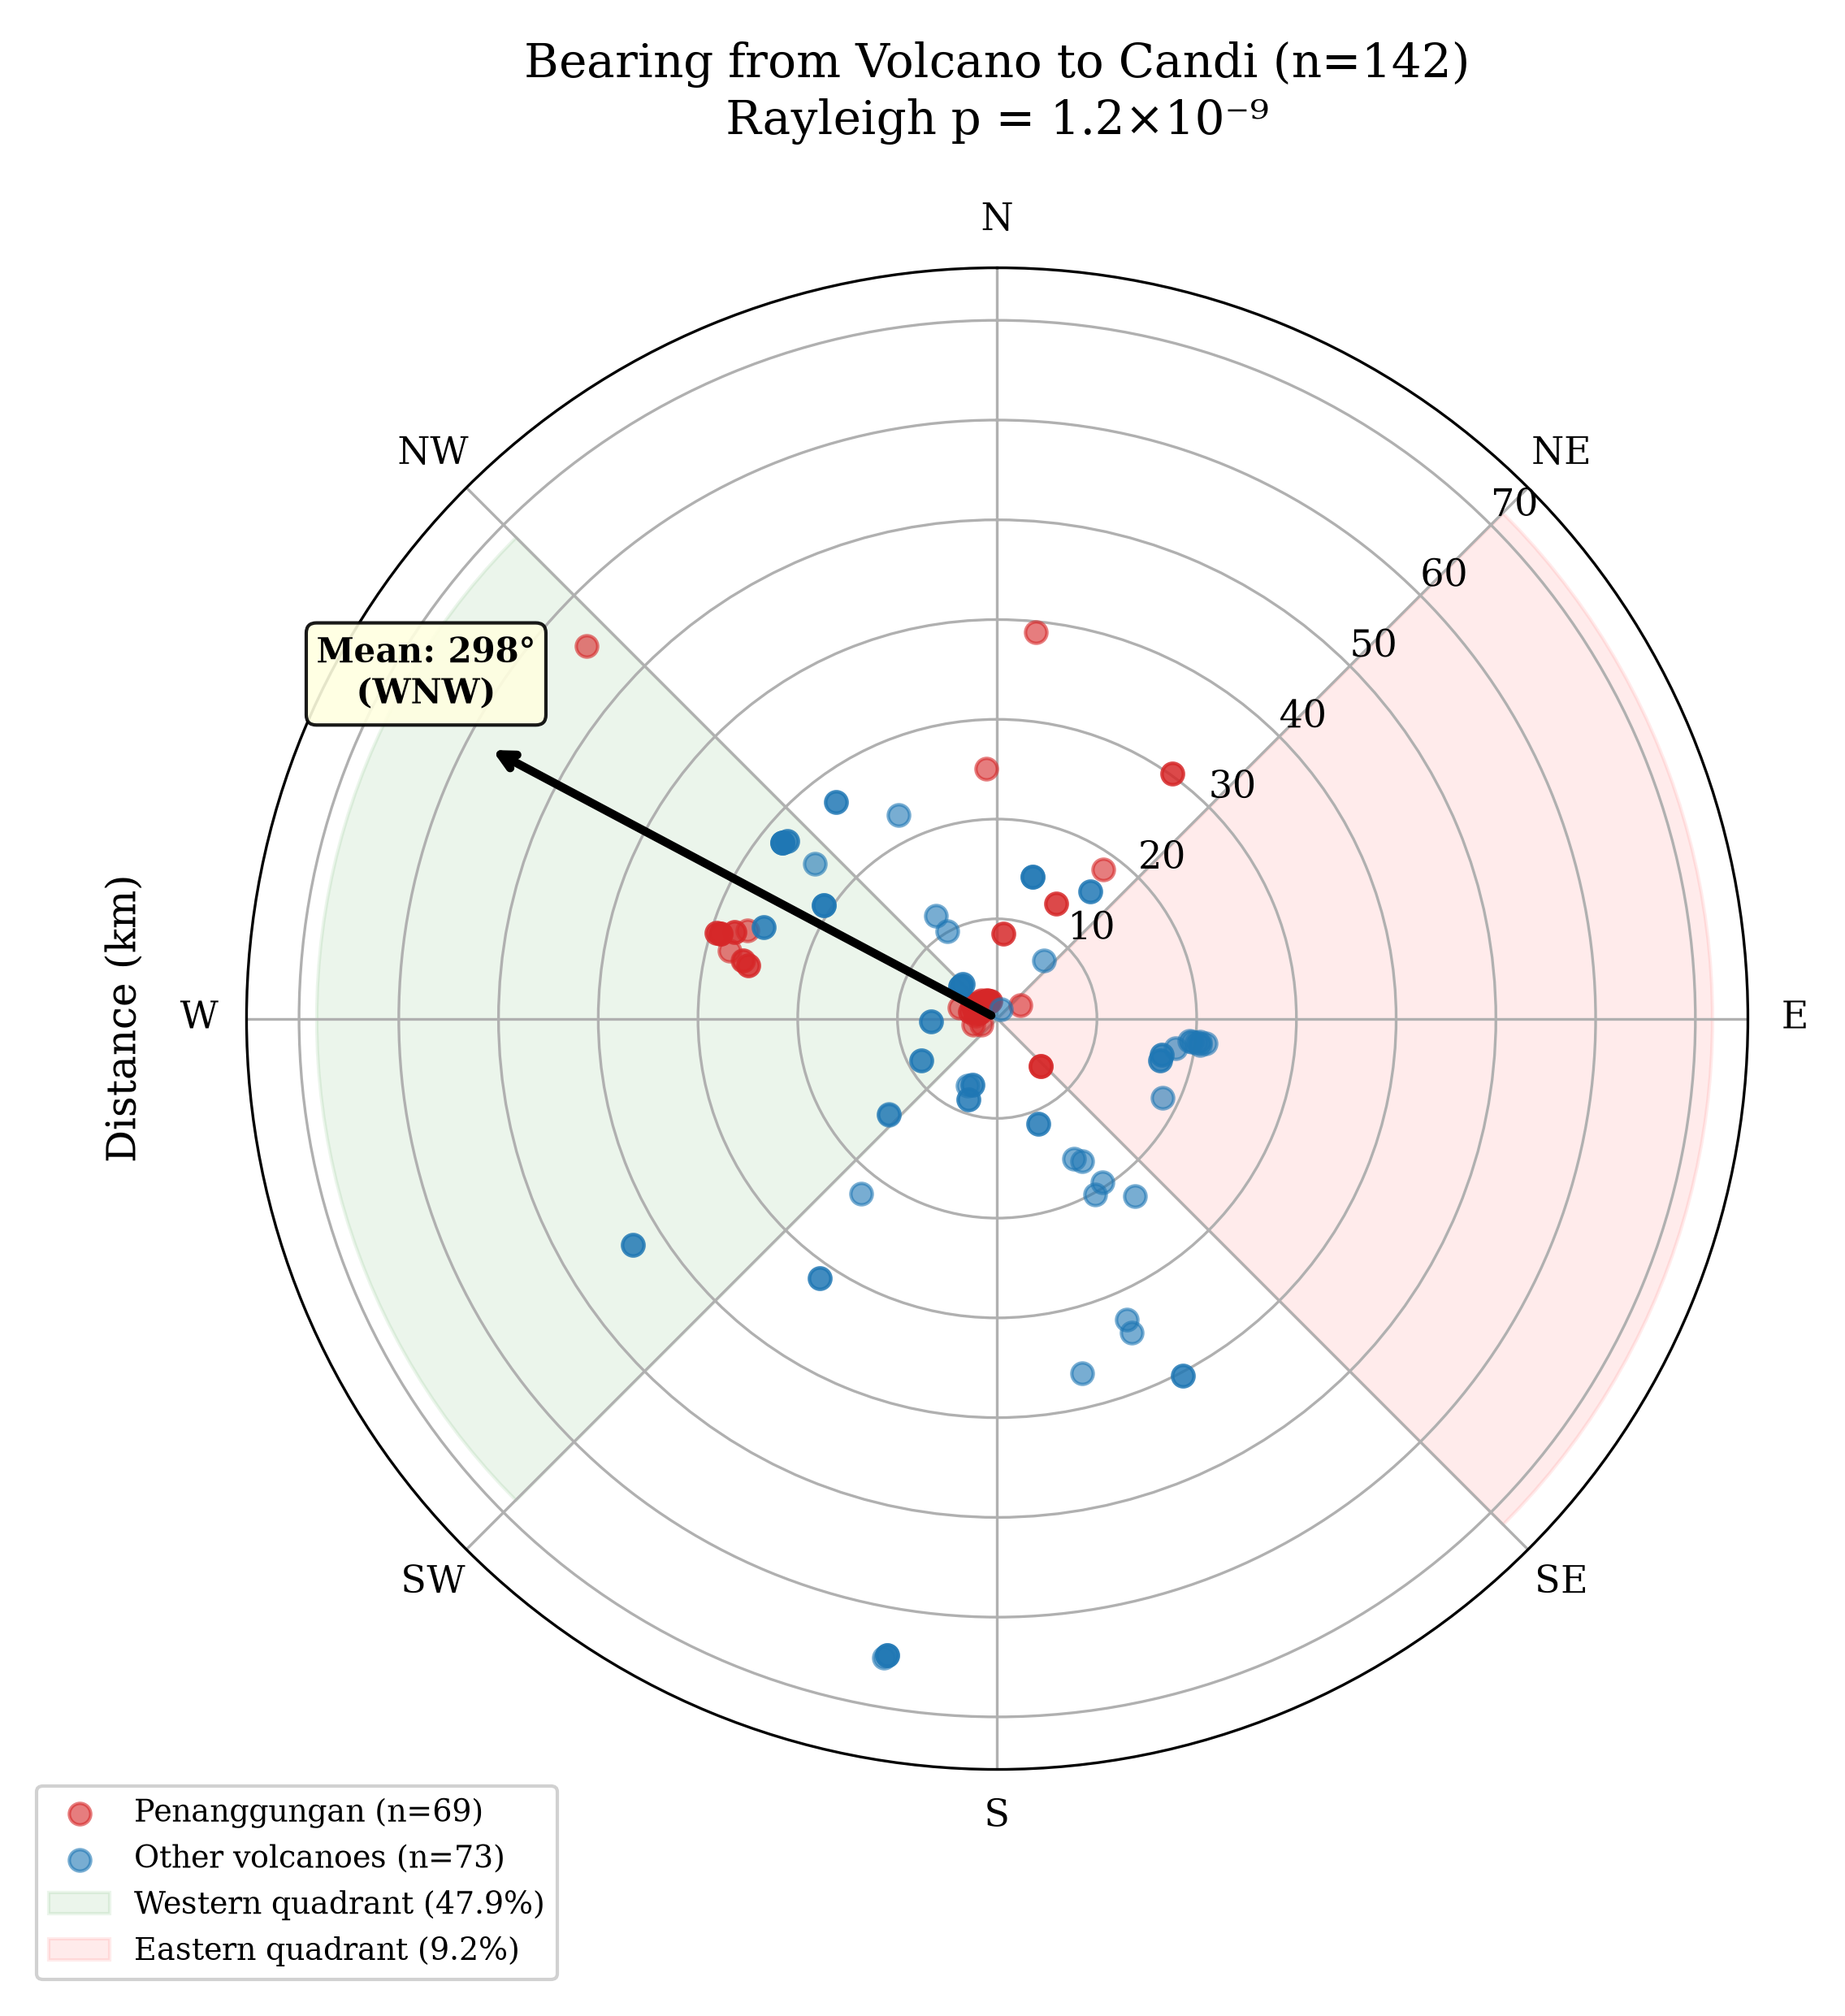
\includegraphics[width=0.7\textwidth]{figures/fig1_candi_polar_bearings.png}
\caption{\textbf{Figure 1.} Polar plot of candi bearings from nearest volcanic peak. The strong western clustering ($279^{\circ}$ mean) is consistent with tephra-sheltered positioning on the leeward side of prevailing eruption plumes.}
\label{fig:polar}
\end{figure}

Quadrant distribution: West 47.2\%, South 26.8\%, North 22.5\%, East 3.5\% ($\chi^2=54.68$, $p<0.0001$). The eastern quadrant is nearly empty: only 5 candi of 142 ($<$4\%).

\begin{table}[h]
\centering
\caption{Candi distribution across volcanic proximity zones}
\small
\begin{tabular}{lrrrr}
\toprule
Zone & Observed & Expected & Ratio & Prediction \\
\midrule
A ($<$10 km) & 60 (42.3\%) & 3.4 & 17.9$\times$ & \textbf{Highest priority} \\
B (10--30 km) & 65 (45.8\%) & 27.0 & 2.4$\times$ & High priority \\
C ($>$30 km) & 17 (12.0\%) & 111.6 & 0.15$\times$ & Low priority \\
\bottomrule
\end{tabular}
\normalsize
\label{tab:zones}
\end{table}

Zone A overrepresentation ($\chi^2=1091.28$, $p<10^{-6}$) indicates that past communities overwhelmingly chose to build within 10~km of volcanic peaks---precisely the zone most affected by sedimentation.

\subsubsection{Penanggungan and Beyond}

Penanggungan alone hosts 73 candi, 46 on the western side (63.0\%; binomial $p<10^{-6}$; Figure~\ref{fig:penanggungan}). Even excluding Penanggungan, the remaining 69 candi still show significant western clustering (Rayleigh $p=0.0009$), confirming that the pattern is not a single-mountain artifact.

\begin{figure}[h]
\centering
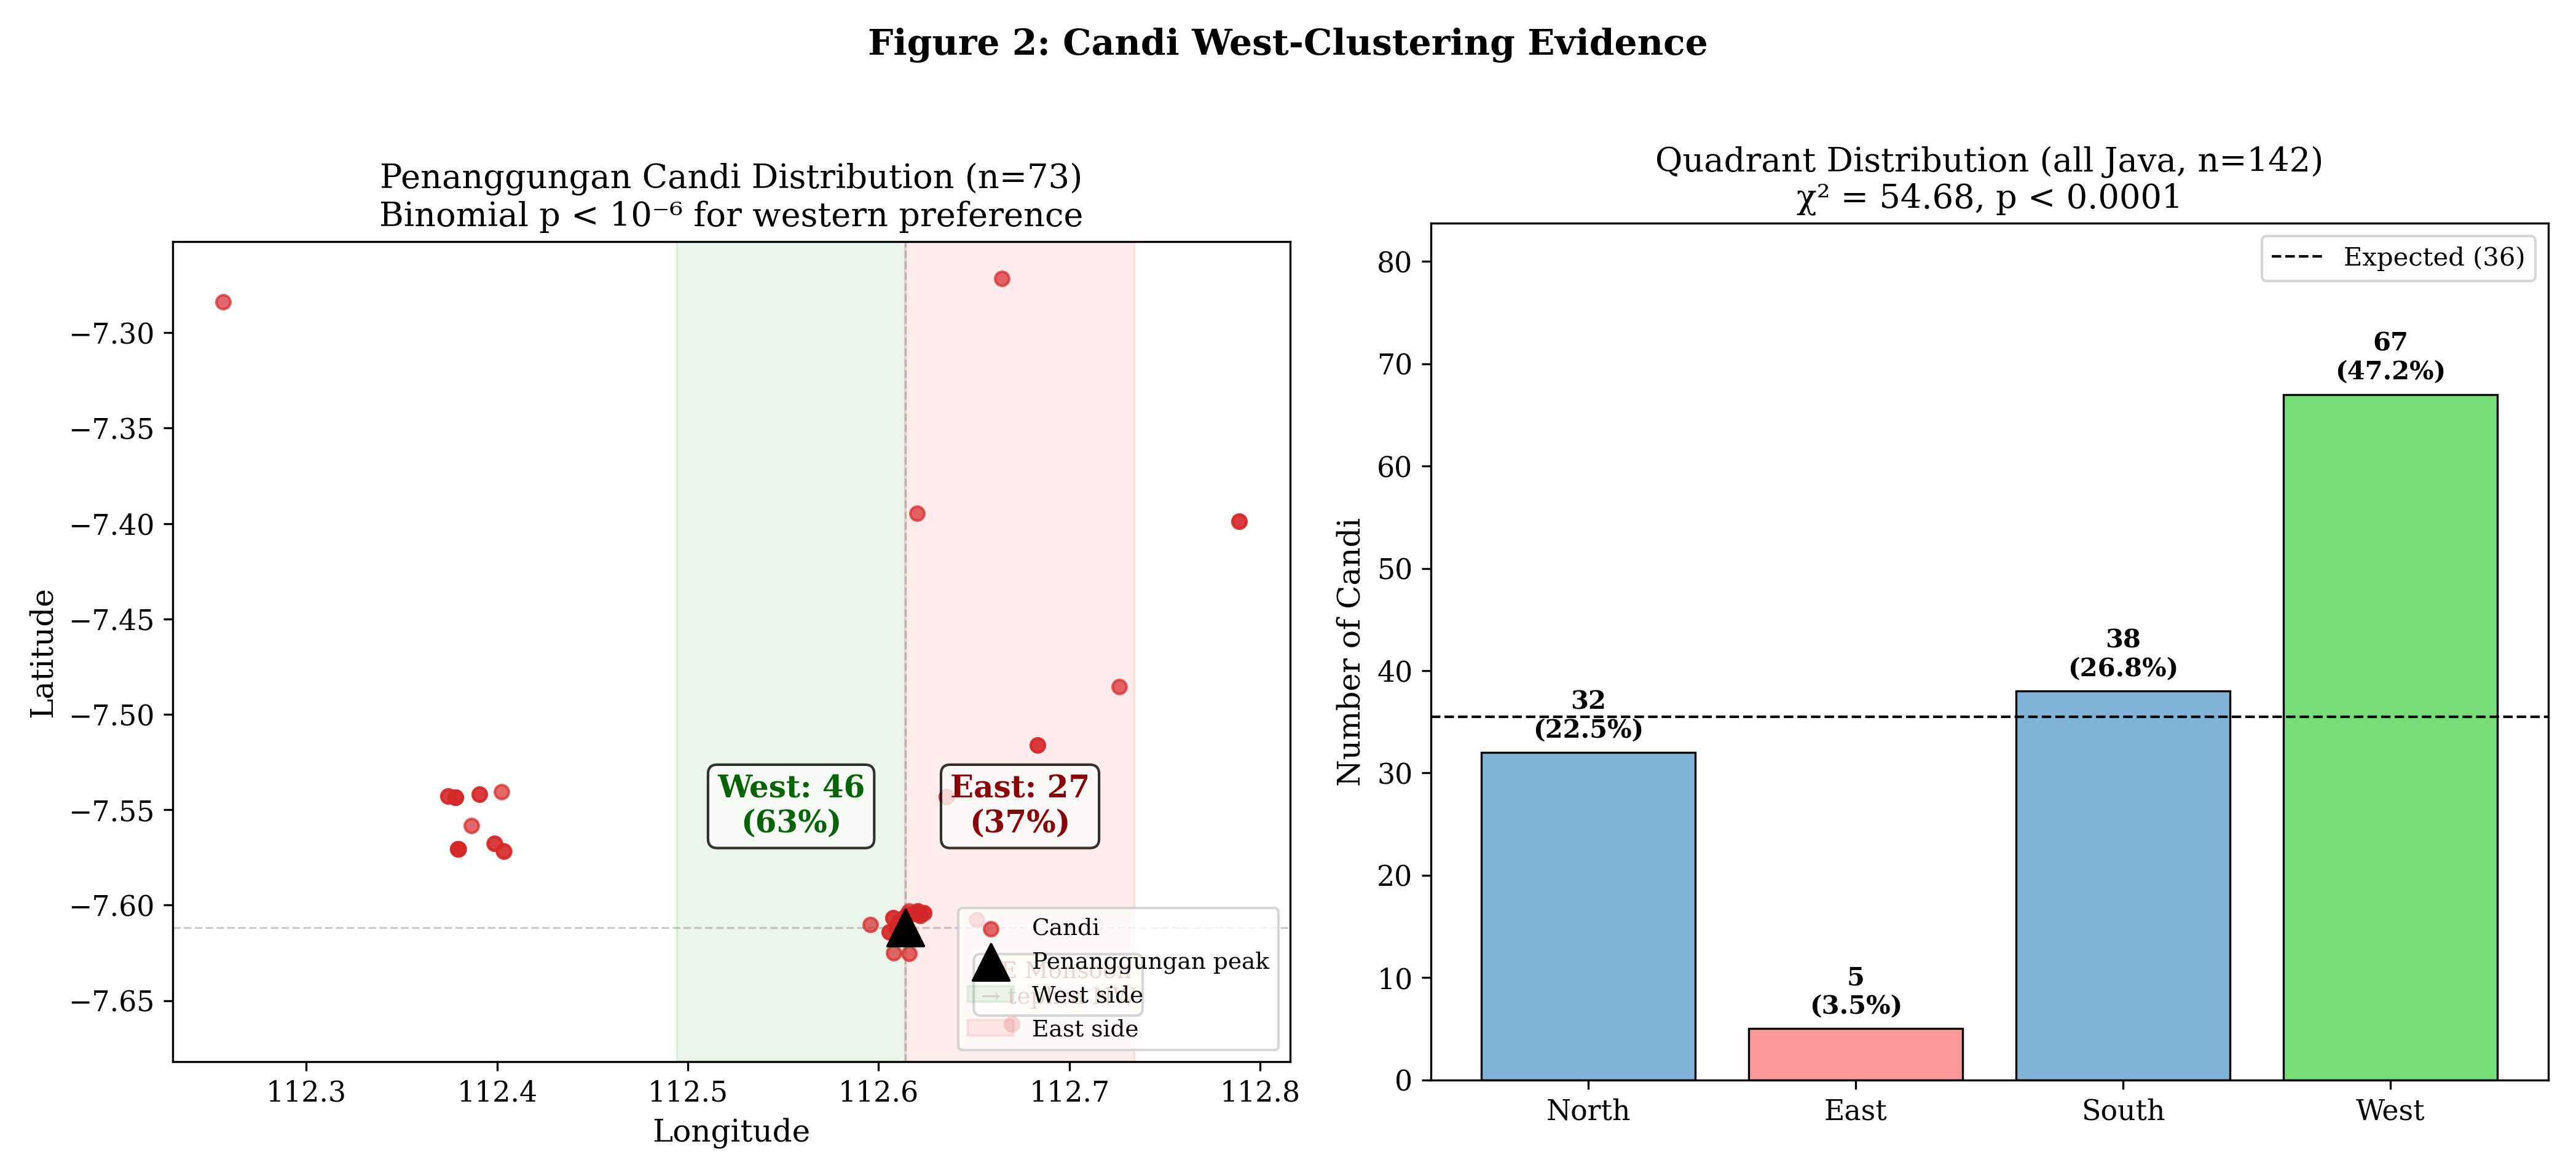
\includegraphics[width=0.7\textwidth]{figures/fig2_penanggungan_westclustering.png}
\caption{\textbf{Figure 2.} Distribution of 73 candi on Penanggungan, showing the 63\% western-flank concentration. The pattern holds for the remaining 69 candi across Java ($p=0.0009$).}
\label{fig:penanggungan}
\end{figure}

\subsection{Inscriptions and Candi Occupy Different Volcanic Zones}

If candi proximity to volcanoes reflected general settlement geography, we would expect inscriptions---which record administrative activity across the inhabited landscape---to show a similar spatial distribution. They do not. Inscriptions are significantly farther from volcanoes than candi (Mann-Whitney $U=16{,}380$, $p=5.2\times10^{-8}$; Kolmogorov-Smirnov $D=0.363$, $p=1.4\times10^{-9}$).

\begin{table}[h]
\centering
\caption{Spatial distribution of candi vs.\ inscriptions relative to nearest active volcano}
\begin{tabular}{lrrrr}
\toprule
 & \multicolumn{2}{c}{Candi ($n=142$)} & \multicolumn{2}{c}{Inscriptions ($n=170$)} \\
\midrule
Zone & $n$ & \% & $n$ & \% \\
\midrule
A ($<$10 km) & 60 & 42.3 & 22 & 12.9 \\
B (10--30 km) & 65 & 45.8 & 111 & 65.3 \\
C ($>$30 km) & 17 & 12.0 & 37 & 21.8 \\
\midrule
Mean distance & \multicolumn{2}{c}{16.5 km} & \multicolumn{2}{c}{25.7 km} \\
Median distance & \multicolumn{2}{c}{14.6 km} & \multicolumn{2}{c}{27.6 km} \\
\bottomrule
\end{tabular}
\label{tab:inscr_candi}
\end{table}

Candi are 3.3$\times$ more concentrated in Zone A than inscriptions ($\chi^2=34.8$, $p=2.8\times10^{-8}$; Fisher's exact for Zone A: OR$=0.20$, $p=6.7\times10^{-9}$). The mean difference of 9.2~km (bootstrap 95\% CI: 5.5--12.7~km) confirms that temple siting reflects a specifically volcanic-proximal behavior distinct from the broader administrative geography recorded in inscriptions.

A temporal dimension reinforces this pattern. Before the 929~CE political migration from Central to East Java, inscriptions average 16.2~km from the nearest volcano (reflecting proximity to Merapi); after 929~CE, inscriptions shift to 38.4~km ($p=5.3\times10^{-8}$). The architectural record, by contrast, maintains volcanic proximity across both periods: candi mean distance to nearest volcano is 16.5~km whether measured for the full dataset or restricted to post-929 East Javanese sites alone (dominated by Penanggungan, mean 7.4~km).

\subsection{Documented Volcanic Burial of Archaeological Sites}

The severity of the taphonomic process that temple siting patterns may reflect is confirmed by 51 documented cases of volcanic burial or destruction of archaeological sites across 12 volcanic systems (Table~\ref{tab:burial}).

\begin{table}[h]
\centering
\caption{Selected archaeological sites buried by volcanic deposits in Java}
\begin{tabular}{llrl}
\toprule
Site & Volcano & Depth (m) & Evidence \\
\midrule
Prambanan Vishnu statue & Merapi & 9.14 & OV 1925 \\
Sambisari & Merapi & 5.00 & 1966 discovery \\
Trowulan deposits & Arjuno-Welirang & 4.28 & OV 1917 \\
Liangan village & Sundoro & 4.00 & 2008 discovery \\
Kedulan & Merapi & 2.70 & 1993 discovery \\
Kelud lahar sites (7 sites) & Kelud & 1.5--2.0 & OV 1919--1920 \\
\bottomrule
\end{tabular}
\label{tab:burial}
\end{table}

The mean burial depth among 24 sites with measured deposits is 3.41~m (median 2.50~m). These depths render sites invisible to surface survey, confirming that the volcanic-zone archaeological deficit reflects genuine burial rather than an absence of past settlement. The Kelud 1919 eruption alone affected seven documented archaeological sites---a single event producing multiple cases of site burial within the study area.

\subsection{Orientation Follows Canon, Not Landscape}

Of 20 candi with documented entrance orientations:
\begin{itemize}
    \item \textbf{85\% face equinox directions} (east or west); binomial $p=4.9\times10^{-14}$
    \item \textbf{100\% on cardinal axes} (N/E/S/W)
    \item Only 35\% face toward the nearest volcano ($p=0.94$, indistinguishable from random)
    \item \textbf{McNemar test} (equinox vs.\ volcano alignment): $\chi^2=10.00$, $p=0.0016$
\end{itemize}

This creates a critical methodological distinction: \emph{where} to build was volcanically informed; \emph{how} to orient was religiously prescribed. Temple siting reflects landscape-level decisions about optimal placement, not random scatter or purely religious considerations. This intentionality is what makes candi distributions usable as predictive proxies.

\subsection{Survey Intensity Does Not Explain the Deficit}
\label{sec:adv3results}

The adversarial regression confirms that the volcanic-zone site deficit is substantive:

\begin{table}[h]
\centering
\caption{Nested Poisson regression: survey intensity vs.\ volcanic proximity}
\begin{tabular}{llrrr}
\toprule
Model & Predictors & Pseudo-$R^2$ & AIC & \\
\midrule
1 (Survey only) & road, BPCB, university & 0.382 & 1373 & \\
2 (Survey + volcanic) & road, BPCB, university, \textbf{volcano} & \textbf{0.398} & \textbf{1340} & \\
\midrule
\multicolumn{4}{l}{Volcanic coefficient: $\beta=-0.477$ (fewer sites near volcanoes)} \\
\multicolumn{4}{l}{Quasi-Poisson LR test: $p=0.0015$ (adjusted for overdispersion $\hat{\phi}=3.55$)} \\
\bottomrule
\end{tabular}
\label{tab:adv3}
\end{table}

Road distance is the dominant predictor ($\beta=-7.15$), confirming that survey access strongly shapes the known site distribution. But after controlling for all three survey proxies, volcanic proximity still explains additional variance. The volcanic-zone deficit is not solely a survey artifact---it reflects genuine site invisibility due to burial.

\subsection{Colonial Calibration Points}
\label{sec:validation}

From colonial OV reports (1912--1929), we extracted 24 measurements of archaeological structures found at depth, including:

\begin{itemize}
    \item Tjandi Tikoes (Trowulan): 3.5~m depth in 1914 ($\sim$5.8~mm/yr if built c.\ 1350~CE)
    \item Submerged city (Trowulan plateau): drainage to 4.28~m required (OV 1920)
    \item Temple structures near Kelud: $>$2~m burial by lahar (OV 1919)
    \item Prambanan area: artifacts at 9.14~m depth (30 voet, Dieduksman collection)
\end{itemize}

These colonial observations independently confirm that archaeological structures in volcanic Java are buried at depths consistent with our sedimentation rate estimates (3--13~mm/yr), and that the burial process was recognized by colonial archaeologists but never systematically analyzed.

% ============================================================
\section{Discussion}
% ============================================================

\subsection{From Pattern to Prediction}

The candi clustering pattern translates directly into fieldwork predictions:

\begin{enumerate}
    \item \textbf{Where to look:} Western flanks of East Java volcanoes, within 10~km of peaks. This zone contains 42\% of all surviving candi but is drastically underrepresented in the modern archaeological site registry.
    \item \textbf{How deep to dig:} Sedimentation rates of 5--13~mm/yr imply that 600-year-old Majapahit-era sites are now 3--8~m below surface, while 1,000-year-old Airlangga-era sites are 5--13~m deep. The colonial depth measurements (3.5--9.1~m) independently confirm this range.
    \item \textbf{What to find:} The ``iceberg principle'' predicts that each surviving candi was surrounded by organic-material settlements (wood, bamboo, thatch) that have been entirely buried. Analysis of 268 DHARMA inscriptions indicates that 63\% of inscribed materials were organic (wood, bamboo, palm leaf), implying that the buried non-monumental record is far larger than the surviving stone record.
\end{enumerate}

\subsection{Liangan as Validation}

The accidental discovery of the Liangan settlement in Central Java in 2008 validates this framework's core prediction \footnote{Novida Abbas, ed., \emph{Liangan: Mozaik Peradaban Mataram Kuno di Lereng Sindoro} (Yogyakarta: Kepel Press / Balai Arkeologi Yogyakarta, 2016).}. Liangan lies 5.5~km from Mount Sindoro on its western flank---Zone~A, the western quadrant---precisely the location class this framework would flag as highest priority. Buried under 6--8~m of pyroclastic deposits, Liangan preserved a complete Mataram-era settlement including wooden houses, carbonised rice grains (tropical japonica), iron-smelting workshops, and Tang Dynasty ceramics---precisely the organic-material domestic infrastructure that candi distributions predict but surface survey cannot detect. Liangan was found by sand miners, not archaeologists, reinforcing the argument that systematic subsurface survey in volcanic Java would recover evidence invisible to current methods.

\subsection{Why This Methodology Works}

Three features make candi distributions particularly reliable as archaeological proxies:

\begin{enumerate}
    \item \textbf{Survival bias works in our favor:} Candi survive precisely because they are stone/brick while surrounding settlements perished. The surviving markers thus indicate the \emph{centers} of now-invisible settlement clusters. A spatial association test confirms this: 81\% of known non-temple archaeological sites (108 sites) lie within 10~km of the nearest candi (mean 6.8~km, Monte Carlo $p<0.0001$), confirming that candi and settlements are spatially co-located, not independent. Epigraphic and archaeological evidence further supports this pattern: Trowulan's urban grid surrounds its candi complexes, and the Prambanan plain preserves both monumental and domestic remains in close proximity.
    \item \textbf{Intentional siting:} The orientation analysis (Section~4.2) confirms that candi placement reflects deliberate landscape decisions. The siting-vs-orientation contrast (McNemar $p=0.0016$) proves that builders considered volcanic topography when choosing locations, making candi positions informationally rich rather than random.
    \item \textbf{Independence from modern survey:} Candi were documented by colonial Dutch archaeologists and are visible as surface features today. Their distribution is thus independent of the modern survey biases that shape the site registry.
\end{enumerate}

\subsection{Comparison with Terrain Suitability Models}

A companion settlement suitability model, developed as part of this project's broader analytical framework (methodology and data available at the project repository), achieved AUC=0.768 for predicting site presence from terrain variables (elevation, slope, river distance). The candi proxy approach is complementary:

\begin{itemize}
    \item The suitability model identifies \emph{where terrain is suitable} for settlement (necessary condition)
    \item The candi proxy identifies \emph{where people actually built} (sufficient evidence)
    \item The intersection---areas that are both terrain-suitable and near candi clusters---represents the highest-confidence prediction zone
\end{itemize}

Ten priority fieldwork targets were derived from this intersection, ranked by predicted burial depth (7--21~m) and proximity to known candi clusters. The top-ranked target (Kelud western flank) has a predicted sedimentation rate of 13.1~mm/yr and is within 2~km of two known Majapahit-era candi. GPS coordinates for all ten targets are available from the corresponding author upon request, in accordance with site protection guidelines.

\subsection{The Japan Comparandum: Volcanism Alone Does Not Create Invisibility}

A potential counter-example is Japan, which has a rich archaeological record in volcanic zones spanning 38,000 years, with $\sim$460,000 registered sites despite hosting 111 active volcanoes. However, Japan's record reflects extraordinary institutional investment: $\sim$8,300 rescue excavations per year (compared to Indonesia's $\sim$70), mandatory developer-funded archaeology since 1950, and per-area survey intensity approximately 100--200$\times$ greater than Indonesia's \footnote{Gina L. Barnes, "Origins of the Japanese Islands: The New `Big Picture,'" \emph{Japan Review} 15 (2003): 3--50. Hiroki Takata and Takahiro Yanase, "Production, Preservation and Dissemination of Archaeological Data in Japan," \emph{Internet Archaeology} 58 (2022).}.

Japan's buried volcanic sites---including settlements sealed by Mt.\ Haruna's 6th-century eruptions at burial depths of $\sim$2~m---were discovered through this rescue system, not through academic surveys \footnote{Satoru Shimoyama, "Volcanic Disasters and Archaeological Sites in Southern Kyushu, Japan," in \emph{Natural Disasters and Cultural Change}, ed. Robin Torrence and John Grattan (London: Routledge, 2002), 326--341.}. The Kikai caldera super-eruption (7,300~BP, VEI-7) makes the point from the opposite direction: it created a demonstrable archaeological gap in southern Kyushu lasting centuries to a millennium, confirming that volcanic events \emph{can} produce temporal voids in the archaeological record.

The Japan comparison clarifies this paper's claims. We do not argue that volcanic burial alone makes civilizations invisible. Rather, volcanic burial combined with insufficient survey intensity renders buried sites undetectable by current methods. Japan has overcome the geological barrier through institutional investment; Indonesia has not. Java's tropical lahar regime further compounds the problem: calibrated sedimentation rates of 2.4--6.2~mm/yr in Java exceed Japan's typical tephra accumulation ($\sim$0.14~mm/yr background) by more than an order of magnitude, driven by monsoonal rainfall that remobilizes volcanic deposits into repeated lahar cycles \footnote{Franck Lavigne and Jean-Claude Thouret, "Sediment Transportation and Deposition by Rain-Triggered Lahars at Merapi Volcano, Central Java, Indonesia," \emph{Geomorphology} 49, no. 1--2 (2003): 45--69.}.

\subsection{Generalizability}

This methodology is not specific to Java. Any volcanic landscape with surviving monumental architecture could apply the same approach:
\begin{itemize}
    \item \textbf{Mesoamerica:} Pyramid distributions relative to Mexican volcanic belt
    \item \textbf{Mediterranean:} Temple distributions near Vesuvius, Etna, Aegean volcanoes
    \item \textbf{Japan:} Shrine distributions relative to the Japanese volcanic arc
\end{itemize}

The key requirement is surviving surface features whose distribution reflects past settlement patterns. In Java, candi fulfill this role; in other contexts, the proxy features may differ. Volcanic preservation of complete settlements has been demonstrated globally---most dramatically at Joya de Cer\'{e}n in El Salvador, where a single eruption (\textasciitilde AD 600) preserved a Maya farming village including thatch roofs, sleeping mats, and food in vessels \footnote{Payson D. Sheets, ed., \emph{Before the Volcano Erupted: The Ancient Cer\'en Village in Central America} (Austin: University of Texas Press, 2002).}. Liangan in Java confirms the same mechanism operates in Southeast Asian volcanic contexts.

\subsection{Limitations}

\begin{enumerate}
    \item \textbf{Penanggungan dominance:} 51\% of candi are on one mountain. While the pattern holds after exclusion ($p=0.0009$), broader spatial coverage would strengthen predictions.
    \item \textbf{No subsurface validation:} All evidence is from surface distributions and colonial observations. Ground-penetrating radar (GPR) or targeted excavation is needed to confirm predictions.
    \item \textbf{Temporal range:} The candi dataset spans c.\ 8th--15th century CE. Predictions for earlier (pre-Hindu) or later (Islamic) periods require different proxy features.
    \item \textbf{Survey proxy crudeness:} Road distance and institutional proximity are imperfect measures of actual survey effort.
    \item \textbf{Sedimentation rate uncertainty:} Colonial depth measurements may reflect localized conditions rather than regional averages.
\end{enumerate}

% ============================================================
\section{Conclusion}
% ============================================================

We demonstrate that the spatial distribution of 142 Hindu-Buddhist candi in Java encodes information about past settlement patterns that can be extracted as predictions for future fieldwork. Four evidence layers converge:

\begin{enumerate}
    \item Candi cluster on western volcanic flanks ($p=3.4\times10^{-8}$) with Zone A ($<$10~km) overrepresented by $17.9\times$, indicating that past settlement concentrated in areas now most affected by volcanic burial.
    \item Comparison with 170 georeferenced inscriptions confirms that this volcanic proximity is specific to sacred architecture ($p=5.2\times10^{-8}$), not a reflection of general settlement geography. Temple siting is a behavioral signal, not a taphonomic artifact.
    \item Fifty-one documented eruption-site correlations with measured burial depths (mean 3.41~m, max 9.14~m) confirm that volcanic burial is severe enough to render sites invisible to surface survey.
    \item An adversarial regression confirms that the volcanic-zone site deficit persists after controlling for survey intensity ($p=0.0015$), and comparison with Japan clarifies that the archaeological gap reflects the \emph{interaction} of volcanic burial with insufficient survey investment.
\end{enumerate}

From these patterns, we derive ten GPS-referenced fieldwork targets with predicted burial depths of 7--21~m. This ``iceberg methodology''---using surviving monumental architecture to locate buried non-monumental remains---offers a cost-effective approach to directing limited survey resources in volcanic terrain. The methodology is generalizable to any volcanic landscape with surviving surface features.

The implication for Java's archaeological record is significant: the areas richest in surviving candi are the same areas where volcanic sedimentation is most intense. The temples are not merely ruins---they are markers of a buried cultural landscape whose recovery requires the kind of systematic investment that Japan's rescue archaeology system demonstrates is possible.

% ============================================================
% DATA AVAILABILITY
% ============================================================

\subsection*{Data Availability}

The candi coordinate dataset, geocoded inscription dataset, tephra-archaeological correlation dataset, and computational scripts used in this study are available at the project repository: \url{https://github.com/neimasilk/volcarch-repo}. Precise GPS coordinates of predicted fieldwork targets are restricted to authorized heritage bodies (BPCB, Balai Arkeologi) to prevent unauthorized excavation.

% ============================================================
% AI DISCLOSURE
% ============================================================

\subsection*{AI Disclosure}

This research used AI tools (Claude, Anthropic) for three tasks: (1) geocoding 182 inscriptions from published findspot descriptions across multiple sources; (2) computing spatial statistics (Rayleigh, Mann-Whitney, Poisson regression, Monte Carlo) on the compiled datasets; and (3) manuscript drafting assistance. Research design, hypothesis formation, data interpretation, and all conclusions are the authors' work. The computational pipeline is available at the project repository.

% ============================================================
% REFERENCES
% ============================================================



\section*{Bibliography}

\noindent Abbas, Novida, ed. \emph{Liangan: Mozaik Peradaban Mataram Kuno di Lereng Sindoro}. Yogyakarta: Kepel Press / Balai Arkeologi Yogyakarta, 2016.

\vspace{0.5em}
\noindent Barnes, Gina L. ``Origins of the Japanese Islands: The New `Big Picture.'\,'' \emph{Japan Review} 15 (2003): 3--50.

\vspace{0.5em}
\noindent DHARMA project. \emph{The Domestication of ``Hindu'' Asceticism and the Religious Making of South and Southeast Asia: Epigraphic Database}. CNRS/ERC, 2024. \url{https://dharma.hypotheses.org/}.

\vspace{0.5em}
\noindent Dumar\c{c}ay, Jacques. \emph{The Temples of Java}. Oxford: Oxford University Press, 1993.

\vspace{0.5em}
\noindent Global Volcanism Program. \emph{Volcanoes of the World}. V. 5.1.1. Smithsonian Institution, 2023. \url{https://volcano.si.edu/}.

\vspace{0.5em}
\noindent Lavigne, Franck, and Jean-Claude Thouret. ``Sediment Transportation and Deposition by Rain-Triggered Lahars at Merapi Volcano, Central Java, Indonesia.'' \emph{Geomorphology} 49, no. 1--2 (2003): 45--69.

\vspace{0.5em}
\noindent Mohr, E. C. J. ``The Relation between Soil and Population Density in the Netherlands East Indies.'' In \emph{Comptes Rendus du Congr\`{e}s International de G\'{e}ographie}. Amsterdam, 1938.

\vspace{0.5em}
\noindent Schiffer, Michael B. \emph{Formation Processes of the Archaeological Record}. Albuquerque: University of New Mexico Press, 1987.

\vspace{0.5em}
\noindent Sheets, Payson D., ed. \emph{Before the Volcano Erupted: The Ancient Cer\'{e}n Village in Central America}. Austin: University of Texas Press, 2002.

\vspace{0.5em}
\noindent Shimoyama, Satoru. ``Volcanic Disasters and Archaeological Sites in Southern Kyushu, Japan.'' In \emph{Natural Disasters and Cultural Change}, edited by Robin Torrence and John Grattan, 326--341. London: Routledge, 2002.

\vspace{0.5em}
\noindent Soekmono, R. \emph{The Javanese Candi: Function and Meaning}. Leiden: Brill, 1995.

\vspace{0.5em}
\noindent Takata, Hiroki, and Takahiro Yanase. ``Production, Preservation and Dissemination of Archaeological Data in Japan.'' \emph{Internet Archaeology} 58 (2022).

\vspace{0.5em}
\noindent Thouret, Jean-Claude. ``Volcanic Geomorphology---an Overview.'' \emph{Earth-Science Reviews} 47, no. 1--2 (1999): 95--131.

\vspace{0.5em}
\noindent Whitten, Tony, Roehayat Emon Soeriaatmadja, and Suraya A. Afiff. \emph{The Ecology of Java and Bali}. Singapore: Periplus Editions, 1996.

\end{document}
